\section{Interacción hombre-máquina y lenguaje natural}
El lenguaje es la capacidad que tiene el ser humano para expresarse y comunicarse a través de diversos sistemas de signos orales, escritos o gestuales. De entre ellos el habla es posiblemente el más complejo pues actúa a diferentes niveles: semántico, lingüístico, articulatorio y sonoro \cite{designTechniques}. Como parte de. Entender correctamente el texto resultante es una tarea igualmente ardua pues el lenguaje va más allá del significado literal de las palabras y por tanto se requiere también una comprensión del contexto en el cual se desarrolla una conversación para interpretarlo correctamente.\\

Con la aparición de nuevas tecnologías y la creciente capacidad de computación se han abierto nuevos campos de investigación de técnicas para el procesamiento de este lenguaje natural (\textit{NLP: Natural language processing}) con el propósito de utilizarlo como medio de interacción entre el hombre y máquina. En los últimos años estos esfuerzos han materializado en el desarrollo de varios sistemas capaces de entender hasta cierto punto las intenciones expresadas por cualquier persona mediante su propia lengua para luego actuar en consecuencia. Si bien estos sistemas utilizan los últimos avances ofrecidos por la inteligencia artificial la realidad es que se encuentran aún en una etapa muy temprana de desarrollo. Aunque pueden interpretar correctamente expresiones bastante difíciles se encuentran aún muy lejos de ofrecer un entendimiento lo suficientemente complejo como para mantener conversaciones naturales y coherentes \cite{designTechniques}. Por tanto, constituyen un punto de partida y sientan las bases del futuro de la interacción entre usuarios y dispositivos, estableciendo un escenario totalmente nuevo donde ya no será necesario utilizar ratón, teclado, pulsaciones o cualquier otra método tradicional de entrada. De hecho, las clásicas interfaces ya están dejando paso a un nuevo paradigma de interacción mucho más intuitivo dónde no es necesario hacer clicks ni teclear datos para realizar ciertas operaciones \cite{conversationSystems}. Por ejemplo, ciertos procesos que antes podían resultar algo tediosos como reservar un vuelo ahora ya son posible con un simple "\textit{Google, resérvame un vuelo a París}", sin necesidad de navegar a través distintas webs ni rellenar formularios.\\

\section{Chatbots}
Un chatbot (\textit{chatter-bot}) o asistente virtual se puede definir como una interfaz (programa) diseñado para que los usuarios puedan interactuar con sus dispositivos haciendo uso de lenguaje natural, ya sea por voz o texto. El objetivo principal es siempre transmitir la sensación al usuario que se encuentra dialogando con una persona real y mantener esta ilusión el mayor tiempo posible. Para ello es crucial que los chatbots sean capaces de demostrar entendimiento, responder con coherencia y resolver las tareas / problemas que los usuarios les planteen.\\

\subsection{Clasificación}
En los últimos años, con la popularización de los chatbots y la democratización de sus tecnologías se han creado multitud de \textit{bots} con propósitos muy distintos. Esto dificulta realizar una clasificación precisa dada la alta subjetividad respecto  al ámbito al cual puede pertenecer un chabot. Sin embargo, es posible realizar una clasificación general en función de los siguientes criterios: Objetivo, modo de interacción, técnica de diseño y ámbito \cite{designTechniques,chatbotTypes}.\\

\subsubsection{Objetivo}
Según el objetivo para el cual han sido diseñados los chatbots pueden clasificarse en:

\begin{itemize}
  \item \textit{Task oriented}: Su objetivo es ayudar a los usuarios a realizar una tarea muy concreta \cite{designTechniques}. En consecuencia, están diseñados para desenvolverse en contextos bastante específicos como reservar un vuelo o anotar un evento en la agenda. En la mayoría de los casos estas acciones han sido establecidas previamente por lo que el flujo de la conversación y todos los posibles caminos están ya previstos \cite{chatbotTypes}.
  \item \textit {Non-task oriented / Conversacionales}: No tienen ningún propósito en particular y su función se limita a mantener una conversación con el usuario. Por ende, su propósito es asemejarse lo máximo a una conversación real respondiendo y siguiendo adecuadamente al interlocutor.
  \item \textit {Informativos}: Son \textit{bots} cuya única tarea es ofrecer al usuario la información que requiera. Normalmente esta información es extraída mediante algoritmos de \textit{string matching} de una base de datos u otra fuente de datos estática. Un ejemplo claro de aplicación son los asistentes que resuelven las dudas más frecuentes (\textit{FAQS}) \cite{chatbotTypes}.
\end{itemize}


\subsubsection{Modo de interacción}
Dependiendo de como el usuario interactúe con el asistente se puede clasificar el chatbot como basado en texto, basado en voz o en respuestas predefinidas. Los siguientes modos no son incompatibles y muchos \textit{bots} combinan ambos.


\begin{itemize}
	\item \textit{Voz}: Aquellos chatbots cuyo método de entrada es la voz. El asistente registra el conjunto de sonidos emitido por el usuario, lo traduce a texto e interpreta su significado. Este es el caso de los famosos asistentes del hogar \textit{Google Home} o \textit{Alexa} dónde por la naturaleza de la aplicación el soporte de voz resulta ser lo más conveniente.
	\item \textit{Texto}: Los \textit{bots} basados en texto aceptan la escritura libre de cualquier mensaje y suelen encontrarse en dispositivos donde escribir resulta cómodo como ordenadores y móviles.
	\item \textit{Respuestas predefinidas}: Dentro de los chatbots basados en texto se encuentran aquellos con los que se interactúa mediante el uso de respuestas predefinidas, normalmente haciendo uso de botones de respuesta rápida. Estos asistentes tienen el flujo de conversación estrictamente definido y por tanto el usuario sólo puede recorrer un número limitado de caminos previamente definidos.
\end{itemize}



\subsubsection{Técnica de diseño}
[TODO: Explicar brevemente técnicas de diseño]
\begin{itemize}
	\item \textit{Basado en reglas}: O \textit{rule based}
	\item \textit{Recuperación}: \textit{retrieval based}
	\item \textit{Generativos}: \textit{generative based} 
\end{itemize}

\subsubsection{Ámbito}
En función del conocimiento que posea el chatbot y los campos que intente abarcar se pueden definir como de ámbito abierto o cerrado.

\begin{itemize}
	\item \textit{Ámbito  abierto}: Asistentes que no tienen una área de conocimiento en específico, tienen un carácter más general y suelen estar hechos para el entretenimiento.
	\item \textit{Ámbito cerrado}: Centrados en resolver dudas o realizar tareas dentro de un ámbito muy específico. Suelen  fallar al responder sobre temas más generales.
\end{itemize}


\begin{figure}[htbp]
\centering
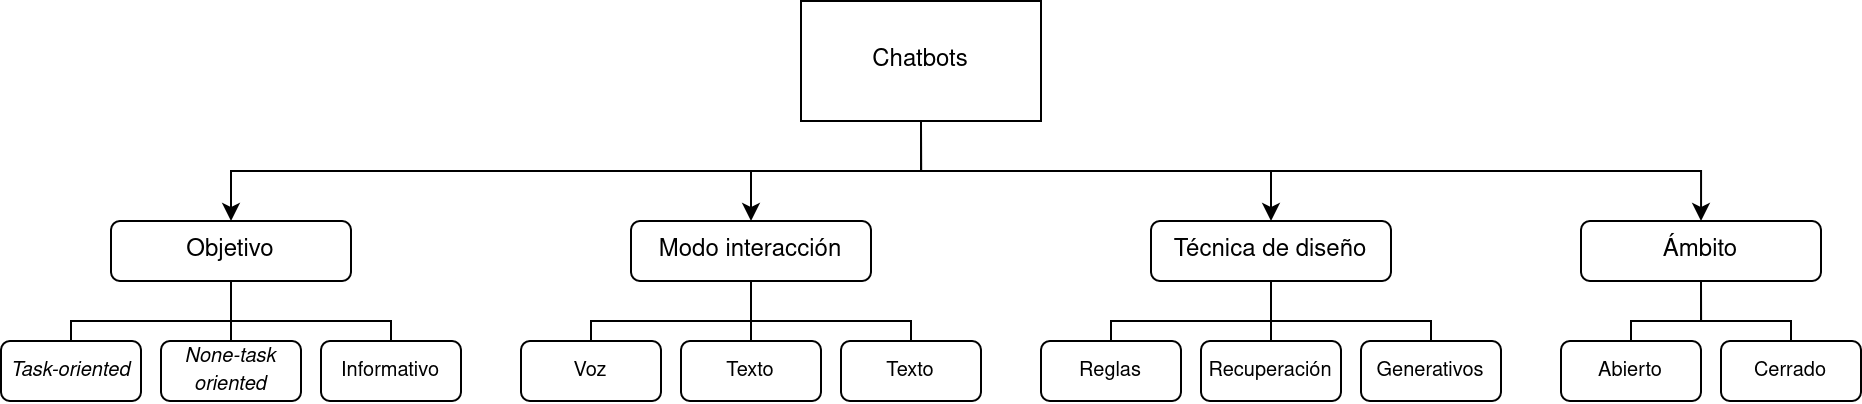
\includegraphics[scale=0.25]{../images/clasificacionChatbots.png} 
\caption{Clasificación de chatbots}
\label{fig:x clasificacion chatbots}
\end{figure}

 
 
\subsection{Técnicas de diseño }
\label{tecnicas diseño}
Para que un chatbot responda de forma adecuada es crucial reconocer que intenciones tiene el usuario cunado se expresa. Para ello, anteriormente se utilizaban algoritmos simples de \textit{pattern matching} para construir sistemas basados en reglas donde la interacción se limitaba a un simple patrón de pregunta-respuesta. Sin embargo, hoy en día con la aparición de nuevas técnicas es posible crear sistemas más complejos que nos permitan implementar patrones de conversación mucho más sofisticados, ofreciendo al usuario final una experiencia mucho más natural, y por lo tanto humana. \\

%la inteligencia artificial nos ha brindado una serie de herramientas muy útiles para para este objetivo: la comprensión del lenguaje natural, consciente del contexto, \textit{machine learning} y  aprendizaje supervisado. \\

[TODO: Desarrollar técnicas de diseño]


\subsection{Interacción y características sociales}
Como ya se ha mencionado, es de vital importancia que las conversaciones entre el \textit{bot} y el usuario sean lo más semejantes posibles a una entre humanos. Para ello no deben de transmitir una sensación robótica, si no que deben ser fluidas y lo más humanas posibles. Para ello, un chatbot debe de integrar una serie de caracterísitcas mínimas que garantizen esta experiencia.\\

[TODO: Desarrollar caracterísitcas sociales y como debe interactuar]


\section{Estado del arte}
Muchas de las tecnologías mencionadas anteriormente se han empezado a introducir en el campo de la medicina y de la salud en busca de soluciones que mejoren la vida de los pacientes. Aprovechando los últimos avances en interacción entre personas y máquinas  se están desarrollando propuestas de asistentes virtuales que ayuden en el día a día a pacientes, familiares o incluso personas mayores. La idea es siempre mejorar la atención y automatizar ciertos procesos médicos \cite{healthAgents} bastante comunes y rutinarios como puedan ser responder a ciertas consultas, realizar el seguimiento de una medicación o detectar principios de enfermedad. \\

\subsection{Chatbots en el campo de la salud}
Dependiendo de la intención y problema que pretendan solucionar en el campo se la salud se diferencian 4 grandes categorías: educación, \textit{coaching}, prevención y diagnóstico.\\

\subsubsection{Educación}
Los chatbots educativos son aquellos orientados a ayudar a los usuarios a entender conceptos médicos y resolver todas aquellas dudas que puedan tener. Esta tarea la pueden realizar proporcionando información relevante sobre cierta enfermedad, resolviendo dudas técnicas sobre un análisis o ayudando a pacientes y familiares a comprender diagnósticos y tratamientos. \\

Por ejemplo, un asistente virtual en este contexto podría resultar útil para  concienciar y advertir a la población sobre los riesgos de una determinada enfermedad . Este es el caso de IRA, un chatbot creado en India que, al igual que Vihrtual-App tiene por objetivo ayudar con en el grave problema padece el país con el VIH ofreciendo información y motivando a la gente a ser conscientes y responsables.\\

\begin{figure}[htbp]
\centering
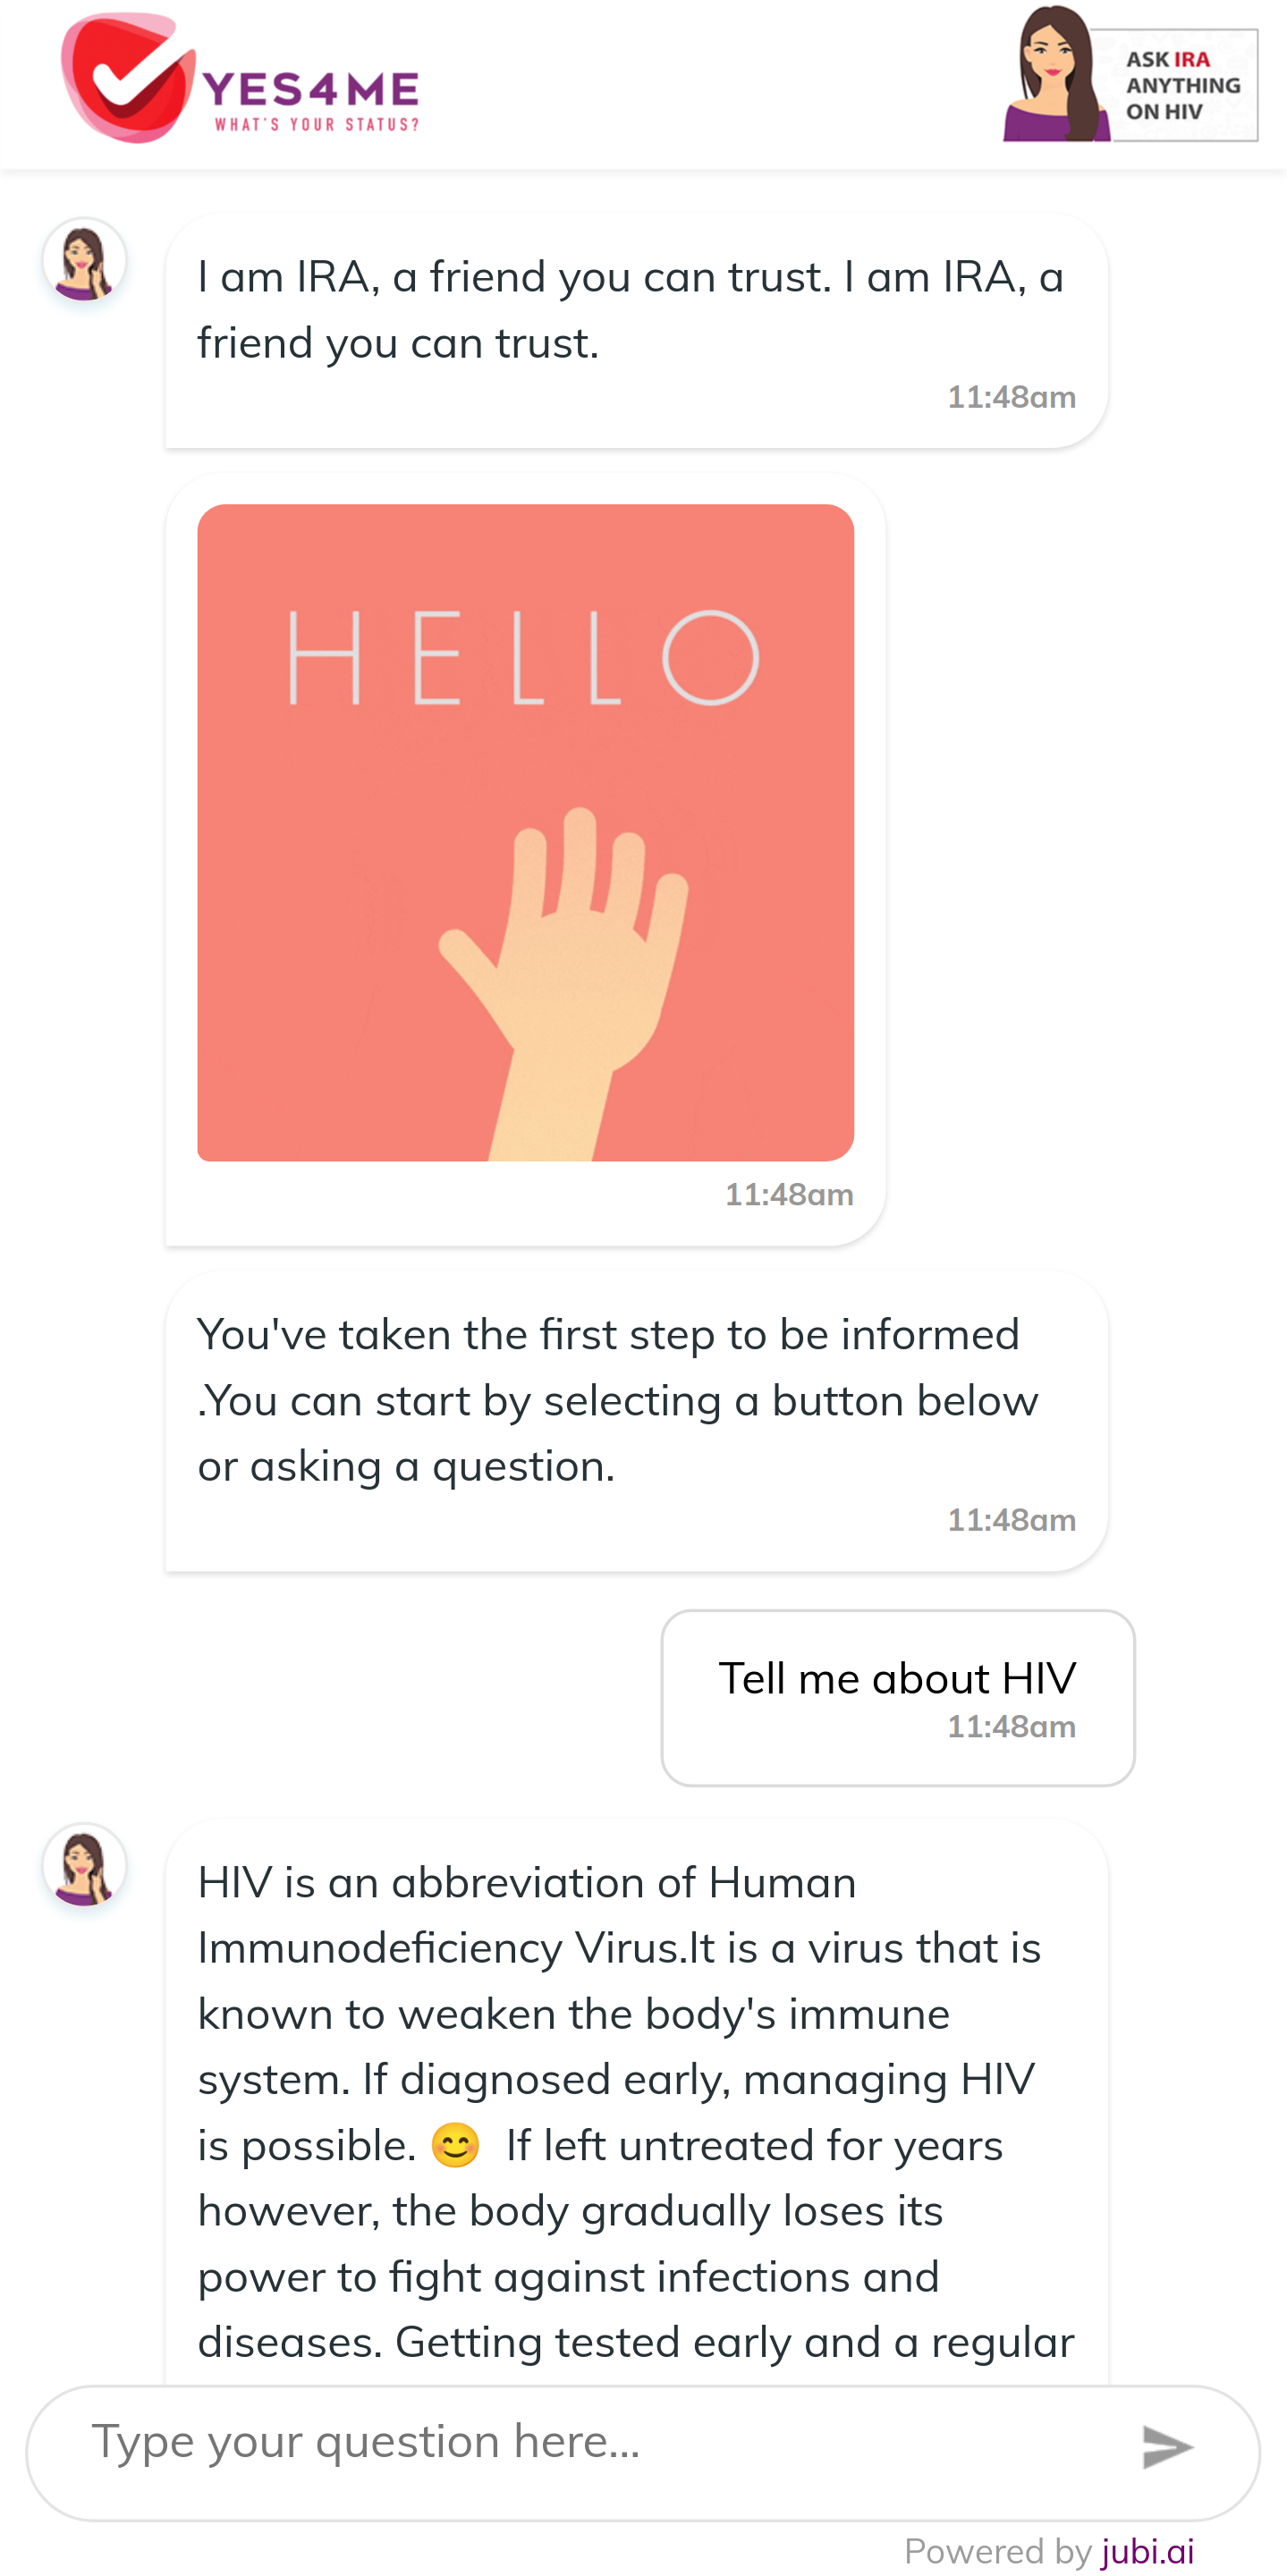
\includegraphics[scale=0.1]{../images/ira.png} 
\caption{Captura de pantalla de IRA}
\label{fig:x captura ira}
\end{figure}

\subsubsection{Coaching}
La segunda categoría hace referencia al término \textit{coach}, que en español significa entrenador personal. Son chatbots similares a los anteriores pues están orientados también a formar al usuario pero, si en el anterior grupo la posición del asistente era bastante pasiva, aquí es todo lo contrario. Este tipo de asistentes toman una actitud de liderazgo para influir y mejorar directamente en la salud del usuario.\\

De esta manera, un chatbot podría enviar notificaciones al móvil de un paciente para recordarle cuándo debe tomar la medicación y así trabajar para introducir nuevos hábitos y comportamientos. También podría aconsejar mejores hábitos de vida y proponer objetivos diarios al usuario, trabajando codo con codo para mejorar su salud.\\

Un buen ejemplo de esta aplicación es Florence, un asistente que pretende ser un enfermero personal que recuerda a los usuarios cuándo deben tomarse la medicación y lleva un seguimiento del peso, presión arterial y periodo.\\

\begin{figure}[htbp]
\centering
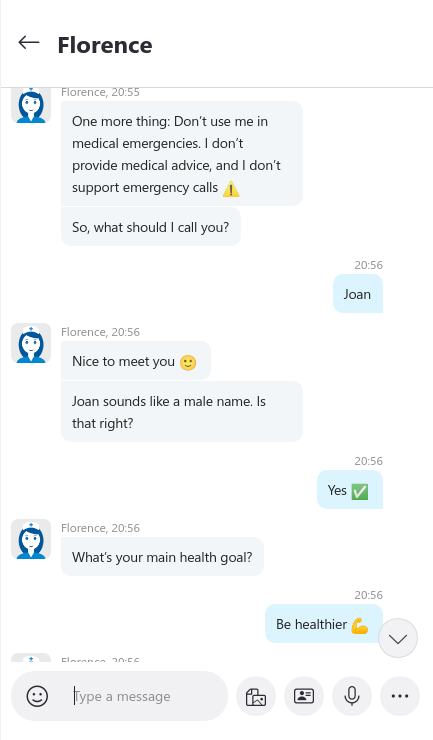
\includegraphics[scale=0.5]{../images/florence.png} 
\caption{Captura de pantalla de Florence}
\label{fig:x captura florence}
\end{figure}

\subsubsection{Prevención}
En la categoría de prevención se engloban todos aquellos chatbots orientados a mantener una relación continua entre médico y paciente. A través de conversaciones rutinarias un asistente virtual puede detectar patrones habituales ya conocidos y anticiparse a cualquier problema que pueda derivar en una posible enfermedad. Por ejemplo, mediante técnicas más avanzadas es posible detectar principios de demencia \cite{detectDementia} o actitudes depresivas para la prevención de suicidios.\\


\subsubsection{Diagnóstico}
Por último, el cuarto grupo son aquellos chatbots que en base a unas indicaciones sintomatológicas es capaz de sugerir un diagnóstico. Esta clase de \textit{bots} suelen utilizarse un ambiente clínico como una herramienta más para los médicos y que, por ejemplo, haciendo uso de grandes bases de datos y estadísticas sugieran al médico posibles diagnósticos.\\

Por otra parte también existen aplicaciones en este sentido donde se usa directamente por usuarios fuera del ámbito médico, y por tanto, suelen ser diagnósticos más sencillos. En esta dirección tarabaja \textit{Wakamola}, un chatbot que, a través de una serie de preguntas recoge información sobre la dieta, actividad física, edad, peso etc. En función de las respuestas del usuario se realiza un cálculo y se muestra una puntuación (\textit{Wakaestado}) entre 0 y 100.

\begin{figure}[htbp]
\centering
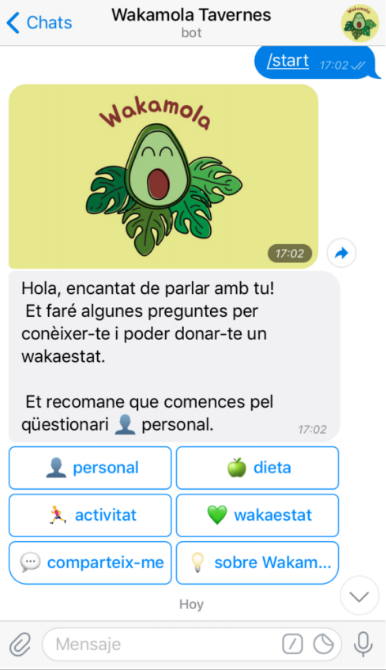
\includegraphics[scale=0.5]{../images/wakamola.png} 
\caption{Captura de pantalla de Wakamola}
\label{fig:x captura wakamola}
\end{figure}

\section{Herramientas para construir chatbots} \label{herramientas construir chatbots}
A la hora de desarrollar un chatbot existen diferentes herramientas que facilitan el uso e implementación de varias de las técnicas descritas en la sección \ref{tecnicas diseño}. A continuación se realiza un análisis y comparativa de las alternativas más relevantes para construir chatbots.\\

\subsection{Rasa}
\textit{Rasa} es un \textit{framework} gratuito y \textit{opensource} que permite construir sistemas conversacionales inteligentes. Esta herramienta proporciona tres grandes funcionalidades para la construcción de un chatbot: comprensión del lenguaje natural (\textit{NLU}), control del flujo los diálogos mediante algoritmos de \textit{machine learning} e integración con distintos canales (\textit{API REST}, aplicaciones de mensajería instantánea etc).\\

\textit{Rasa} hace una fuerte apuesta por el desarrollo basado en conversaciones reales (\textit{CDD: Conversation driven development}) y para ello ofrece un producto gratuito llamado \textit{Rasa X}. Aunque no es \textit{opensource} sí es gratuito y de libre uso facilitando la recogida y posterior etiquetado de las conversaciones.\\

\subsection{Amazon Lex}
Amazon Lex es un servicio para crear agentes conversacionales que interactúen mediante voz o texto. Esta tecnología es la misma que se encuentra detrás de \textit{Alexa}, por tanto este servicio pone a disposición de los desarrolladores el propio motor del popular asistente de Amazon.\\

Las principales características que ofrece son comprensión del lenguaje natural (NLU), reconocimiento automático de voz (ASR) e integración con distintos canales. El uso de la voz y la potencia de motor permite construir experiencias muy atractivas pero por contra, el servicio hace uso de los sistemas en la nube y cobra por cada solicitud de texto o voz que se realice (3.25€ por cada 1000 peticiones de voz y 0.60€ por cada 1000 de texto).\\

\subsection{Microsoft Bot Framework}


\subsection{Botkit}


\begin{table}[htbp]
\centering
\begin{tabular}{|l|l|l|l|l|} 
\hline
                   & Microsoft & Botkit   & Amazon Lex & Rasa      \\ 
\hline
Basado en la nube  & Sí        & Sí       & Sí         & No        \\ 
\hline
NLP                & Sí        & No       & Sí         & Sí        \\ 
\hline
Soporte mensajería & Sí        & Sí       & Sí         & Sí        \\ 
\hline
Coste              & Pago      & Gratuito & Pago       & Gratuito  \\
\hline
\end{tabular}
\caption{Comparativa de \textit{frameworks}}
\end{table}


